\documentclass[a4]{article}

\usepackage[T1]{fontenc}
\usepackage[icelandic]{babel}
\usepackage{amsmath}
\usepackage{graphicx}
\usepackage{sidecap}
\usepackage[utf8]{inputenc}
%\usepackage[left=1in,top=1in,right=1in,bottom=1in,nohead]{geometry}
\usepackage[framed,numbered,autolinebreaks,useliterate]{../mcode}
\usepackage{amsfonts}
\usepackage{epstopdf}

\lstset{language=MATLAB}

\title{Athugasemdir frá Ragnari\\ Heimaverkefni 3}
\begin{document}
\maketitle
\section{10. apr 2013}

$$\theta''(t) = \frac{g}{s(t)} \cdot \theta(t)$$
$$\theta''(t) = \frac{g}{s(t)} \cdot \sin{\theta(t)}$$

$$T = 2\pi \sqrt{\frac{l}{g}} \cdot \left( 1 + \frac{\theta_0^2}{16} + \ldots \right)$$
Til að bremsa, lengja á niðurleið
\begin{figure}
  \caption{Hvernig s(t) er flott ad hafa i.e. byrja venjulega en svo fara ad rola ser.}
  \centerline{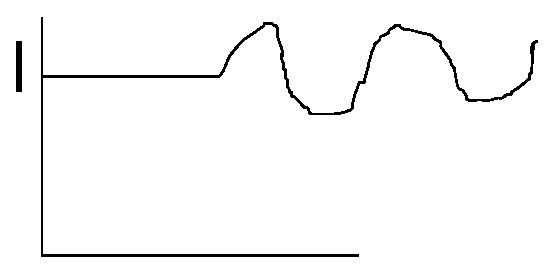
\includegraphics[scale=0.5]{timaath.eps}}
\end{figure}

$$ s = l(1 +a \cos{\omega_0 \cdot t - p})$$
\end{document}